\documentclass[journal,12pt,twocolumn]{IEEEtran}

\usepackage{setspace}
\usepackage{gensymb}

\singlespacing


\usepackage[cmex10]{amsmath}

\usepackage{amsthm}

\usepackage{mathrsfs}
\usepackage{txfonts}
\usepackage{stfloats}
\usepackage{bm}
\usepackage{cite}
\usepackage{cases}
\usepackage{subfig}

\usepackage{longtable}
\usepackage{multirow}

\usepackage{enumitem}
\usepackage{mathtools}
\usepackage{steinmetz}
\usepackage{tikz}
\usepackage{circuitikz}
\usepackage{verbatim}
\usepackage{tfrupee}
\usepackage[breaklinks=true]{hyperref}
\usepackage{graphicx}
\usepackage{tkz-euclide}
\usepackage{float}

\usetikzlibrary{calc,math}
\usepackage{listings}
    \usepackage{color}                                            %%
    \usepackage{array}                                            %%
    \usepackage{longtable}                                        %%
    \usepackage{calc}                                             %%
    \usepackage{multirow}                                         %%
    \usepackage{hhline}                                           %%
    \usepackage{ifthen}                                           %%
    \usepackage{lscape}     
\usepackage{multicol}
\usepackage{chngcntr}

\DeclareMathOperator*{\Res}{Res}

\renewcommand\thesection{\arabic{section}}
\renewcommand\thesubsection{\thesection.\arabic{subsection}}
\renewcommand\thesubsubsection{\thesubsection.\arabic{subsubsection}}

\renewcommand\thesectiondis{\arabic{section}}
\renewcommand\thesubsectiondis{\thesectiondis.\arabic{subsection}}
\renewcommand\thesubsubsectiondis{\thesubsectiondis.\arabic{subsubsection}}


\hyphenation{op-tical net-works semi-conduc-tor}
\def\inputGnumericTable{}                                 %%

\lstset{
%language=C,
frame=single, 
breaklines=true,
columns=fullflexible
}
\begin{document}
\newtheorem{theorem}{Theorem}[section]
\newtheorem{problem}{Problem}
\newtheorem{proposition}{Proposition}[section]
\newtheorem{lemma}{Lemma}[section]
\newtheorem{corollary}[theorem]{Corollary}
\newtheorem{example}{Example}[section]
\newtheorem{definition}[problem]{Definition}

\newcommand{\BEQA}{\begin{eqnarray}}
\newcommand{\EEQA}{\end{eqnarray}}
\newcommand{\define}{\stackrel{\triangle}{=}}
\bibliographystyle{IEEEtran}
\providecommand{\mbf}{\mathbf}
\providecommand{\pr}[1]{\ensuremath{\Pr\left(#1\right)}}
\providecommand{\qfunc}[1]{\ensuremath{Q\left(#1\right)}}
\providecommand{\sbrak}[1]{\ensuremath{{}\left[#1\right]}}
\providecommand{\lsbrak}[1]{\ensuremath{{}\left[#1\right.}}
\providecommand{\rsbrak}[1]{\ensuremath{{}\left.#1\right]}}
\providecommand{\brak}[1]{\ensuremath{\left(#1\right)}}
\providecommand{\lbrak}[1]{\ensuremath{\left(#1\right.}}
\providecommand{\rbrak}[1]{\ensuremath{\left.#1\right)}}
\providecommand{\cbrak}[1]{\ensuremath{\left\{#1\right\}}}
\providecommand{\lcbrak}[1]{\ensuremath{\left\{#1\right.}}
\providecommand{\rcbrak}[1]{\ensuremath{\left.#1\right\}}}
\theoremstyle{remark}
\newtheorem{rem}{Remark}
\newcommand{\sgn}{\mathop{\mathrm{sgn}}}
\providecommand{\abs}[1]{\vert#1\vert}
\providecommand{\res}[1]{\Res\displaylimits_{#1}} 
\providecommand{\norm}[1]{\lVert#1\rVert}
%\providecommand{\norm}[1]{\lVert#1\rVert}
\providecommand{\mtx}[1]{\mathbf{#1}}
\providecommand{\mean}[1]{E[ #1 ]}
\providecommand{\fourier}{\overset{\mathcal{F}}{ \rightleftharpoons}}
%\providecommand{\hilbert}{\overset{\mathcal{H}}{ \rightleftharpoons}}
\providecommand{\system}{\overset{\mathcal{H}}{ \longleftrightarrow}}
	%\newcommand{\solution}[2]{\textbf{Solution:}{#1}}
\newcommand{\solution}{\noindent \textbf{Solution: }}
\newcommand{\cosec}{\,\text{cosec}\,}
\providecommand{\dec}[2]{\ensuremath{\overset{#1}{\underset{#2}{\gtrless}}}}
\newcommand{\myvec}[1]{\ensuremath{\begin{pmatrix}#1\end{pmatrix}}}
\newcommand{\mydet}[1]{\ensuremath{\begin{vmatrix}#1\end{vmatrix}}}
\numberwithin{equation}{subsection}
\makeatletter
\makeatother
\let\StandardTheFigure\thefigure
\let\vec\mathbf
\renewcommand{\thefigure}{\theproblem}
\def\putbox#1#2#3{\makebox[0in][l]{\makebox[#1][l]{}\raisebox{\baselineskip}[0in][0in]{\raisebox{#2}[0in][0in]{#3}}}}
     \def\rightbox#1{\makebox[0in][r]{#1}}
     \def\centbox#1{\makebox[0in]{#1}}
     \def\topbox#1{\raisebox{-\baselineskip}[0in][0in]{#1}}
     \def\midbox#1{\raisebox{-0.5\baselineskip}[0in][0in]{#1}}
\vspace{3cm}
\title{ASSIGNMENT 3}
\author{Vaibhav Chhabra\\ AI20BTECH11022}
\maketitle
\newpage
\bigskip
\renewcommand{\thefigure}{\theenumi}
\renewcommand{\thetable}{\theenumi}
Download all python codes from 
\begin{lstlisting}
    https://github.com/vaibhavchhabra25/EE3900-course/blob/main/Assignment-3/codes
\end{lstlisting}
%
and latex-tikz codes from 
%
\begin{lstlisting}
    https://github.com/vaibhavchhabra25/EE3900-course/blob/main/Assignment-3/main.tex
\end{lstlisting}
%
\section{Problem}
(Ramsey-4.2-Tangent and Normal-Q.21)\\
Verify that the perpendicular bisector of the chord joining two points $\vec{x_1}$,$\vec{x_2}$ on the circle
\begin{align}
    \vec{x}^\top\vec{x}+2\myvec{g&f}\vec{x}+c=0
\end{align}
passes through the centre.
\section{Solution}
Since $\vec{x_1}$ and $\vec{x_2}$ lie on the circle,
\begin{align}
       \vec{x_1}^\top\vec{x_1}+2\myvec{g&f}\vec{x_1}+c=0\\
       \vec{x_2}^\top\vec{x_2}+2\myvec{g&f}\vec{x_2}+c=0
\end{align}
Subtracting the two, we get,
\begin{align}
    \vec{x_2}^\top\vec{x_2}-\vec{x_1}^\top\vec{x_1}=-2\myvec{g&f}(\vec{x_2}-\vec{x_1}) \label{a}
\end{align}
The midpoint of the chord $\vec{x_1x_2}$ is 
\begin{align}
    \vec{M}=\dfrac{\vec{x_1}+\vec{x_2}}{2}
\end{align}
Since perpendicular bisector of $\vec{x_1x_2}$ is perpendicular to $\vec{x_1x_2}$ and passes through $\vec{M}$, any general point $\vec{P}$ on the perpendicular bisector can be given using the relation
\begin{align}
    &\left(\vec{x_2}-\vec{x_1}\right)^\top\left(\vec{P}-\vec{M}\right)=0\\
    \implies &\left(\vec{x_2}-\vec{x_1}\right)^\top\vec{P}-\left(\vec{x_2}^\top-\vec{x_1}^\top\right)\left(\dfrac{\vec{x_1}+\vec{x_2}}{2}\right)=0\\
    \implies &\left(\vec{x_2}-\vec{x_1}\right)^\top\vec{P}=\dfrac{\vec{x_2}^\top\vec{x_2}-\vec{x_1}^\top\vec{x_1}+\vec{x_2}^\top\vec{x_1}-\vec{x_1}^\top\vec{x_2}}{2}
\end{align}
Since $\vec{x_1}^\top\vec{x_2}=\vec{x_2}^\top\vec{x_1}$, the equation reduces to
\begin{align}
    2\left(\vec{x_2}-\vec{x_1}\right)^\top\vec{P}=\vec{x_2}^\top\vec{x_2}-\vec{x_1}^\top\vec{x_1}
\end{align}
Using \eqref{a}, we get
\begin{align}
    2\left(\vec{x_2}-\vec{x_1}\right)^\top\vec{P}&=-2\myvec{g&f}(\vec{x_2}-\vec{x_1})\\
    \implies \left(\vec{x_2}-\vec{x_1}\right)^\top\vec{P}&=\left(\vec{x_2}-\vec{x_1}\right)^\top\myvec{-g\\-f}
\end{align}
Since the centre of the circle is $\vec{C}=\myvec{-g\\-f}$, we can clearly see that $\vec{P}=\vec{C}$ satisfies the equation of perpendicular bisector.\\

Hence, the perpendicular bisector of any chord of a circle passes through the centre of the circle.\\

For example, consider the circle
\begin{align}
    \vec{x}^\top\vec{x}+2\myvec{-4&-5}\vec{x}+5=0
\end{align}
and let $\vec{x_1}=\myvec{0\\5-2\sqrt{5}}$ and $\vec{x_2}=\myvec{-2\\5}$.
We can clearly see in the figure that the perpendicular bisector the chord $\vec{x_1x_2}$ passes through the centre of the circle.

\begin{figure}[h!]
    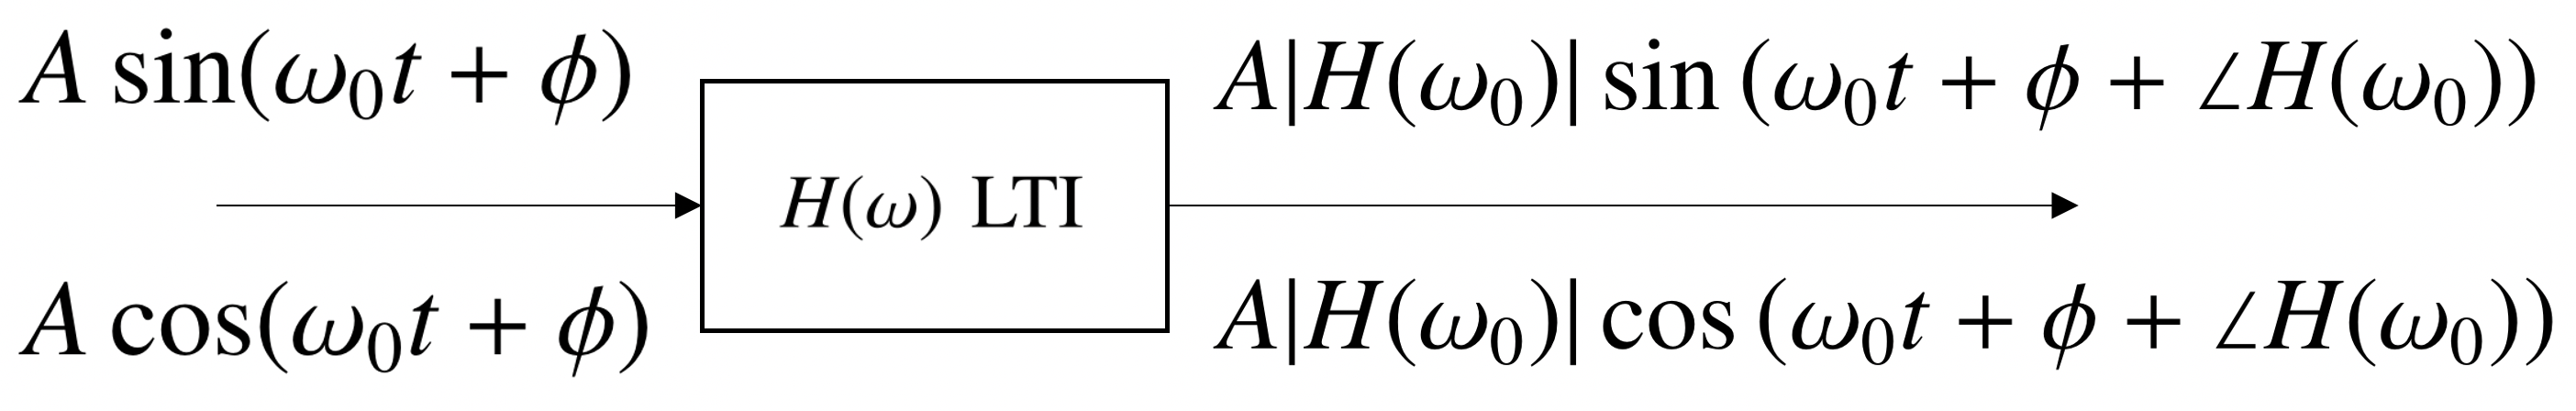
\includegraphics[width=\columnwidth]{figure.png}
    \caption{Example figure}
\end{figure}

\end{document}
